\section{Measurements}
\label{sec:measurements}

\subsection{Controlling the setup with the oscilloscope}
\label{ssub:Controlling the setup with the oscilloscope}
\paragraph{First we measured the}
signal from the detector and photomultiplier. We noticed peaks at irregular points in time 
as can be seen in figure \ref{fig:osci_signal}. Next, the uni- and bipolar signals of the MA are 
examined (see an example in figure \ref{fig:uni_bipolar}). 
The parameters set at the MA are shown in the appendix, table~\ref{tab:config}. 

We can read out rise and fall times for the signal, 
defined as time between 10\% and 90\% of the amplitude and vice verse. 
\begin{itemize}
    \item
        Bipolar:    rise time = $(600 \pm 50)$ ns, fall time $(400 \pm 50)$ ns;
    \item
        Unipolar:   rise time = $(800 \pm 50)$ ns, fall time $(1400 \pm 100)$ ns.
\end{itemize}
Without further information about the activity of the probe, we cannot give a statement about 
possible overlapping of signals. Referring to the prior plot of the peaks distributed in time, we 
assume the probablity of overlapping signals to be low enough, though. 
It is further apparent that the bipolar signal has a much higher resolution in time and is therefore 
more suitable for the time sensitive measurement of delayed coincidences. 
We changed the input from the left to the right detector but did not observe a appreciable differences.
Rotating the sample did not change the result significantly, either.  
\\\\
\begin{SCfigure}
    \begin{centering}
        \caption{
            Events detected by the right detector over a range of 6 ms. 
            The decline rate of 200 $\mu$s is fast enough to evade the 
            coincidence of two events at the given rate. 
            }
        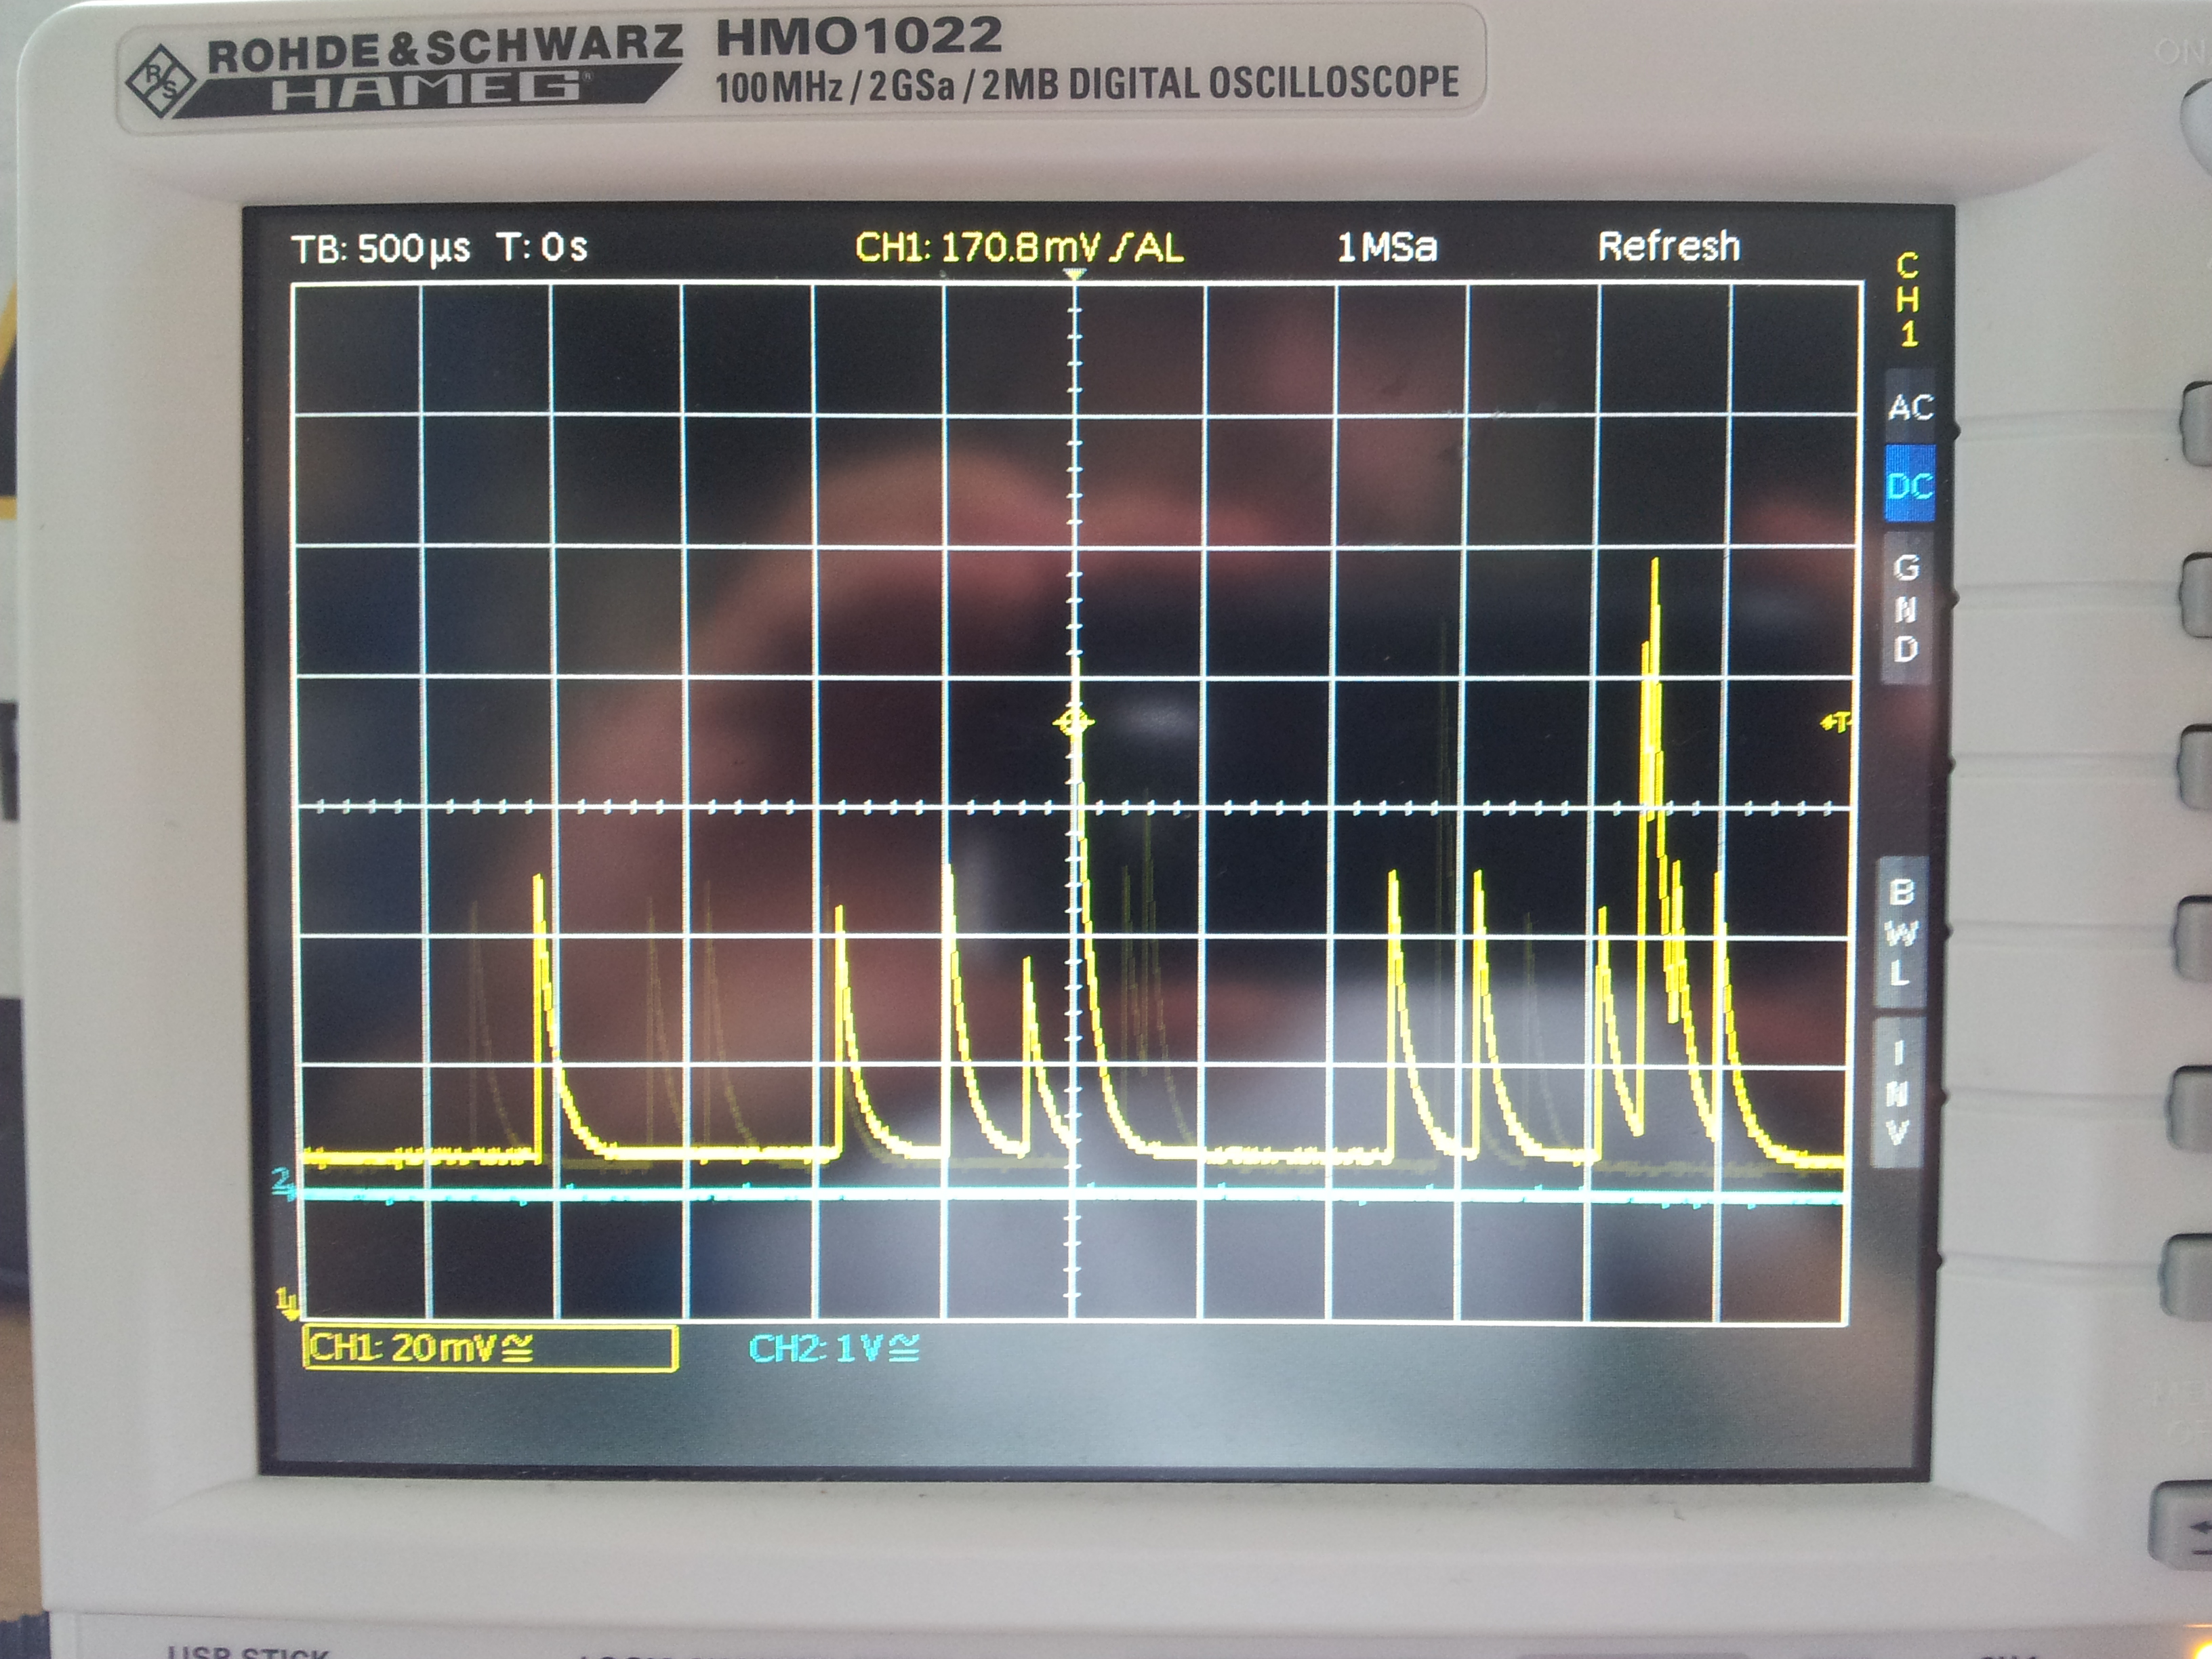
\includegraphics[width=0.45\linewidth]{figures/osci_signal}
        \label{fig:osci_signal}
    \end{centering}
\end{SCfigure}

\begin{figure}[htpb]
    \centering
    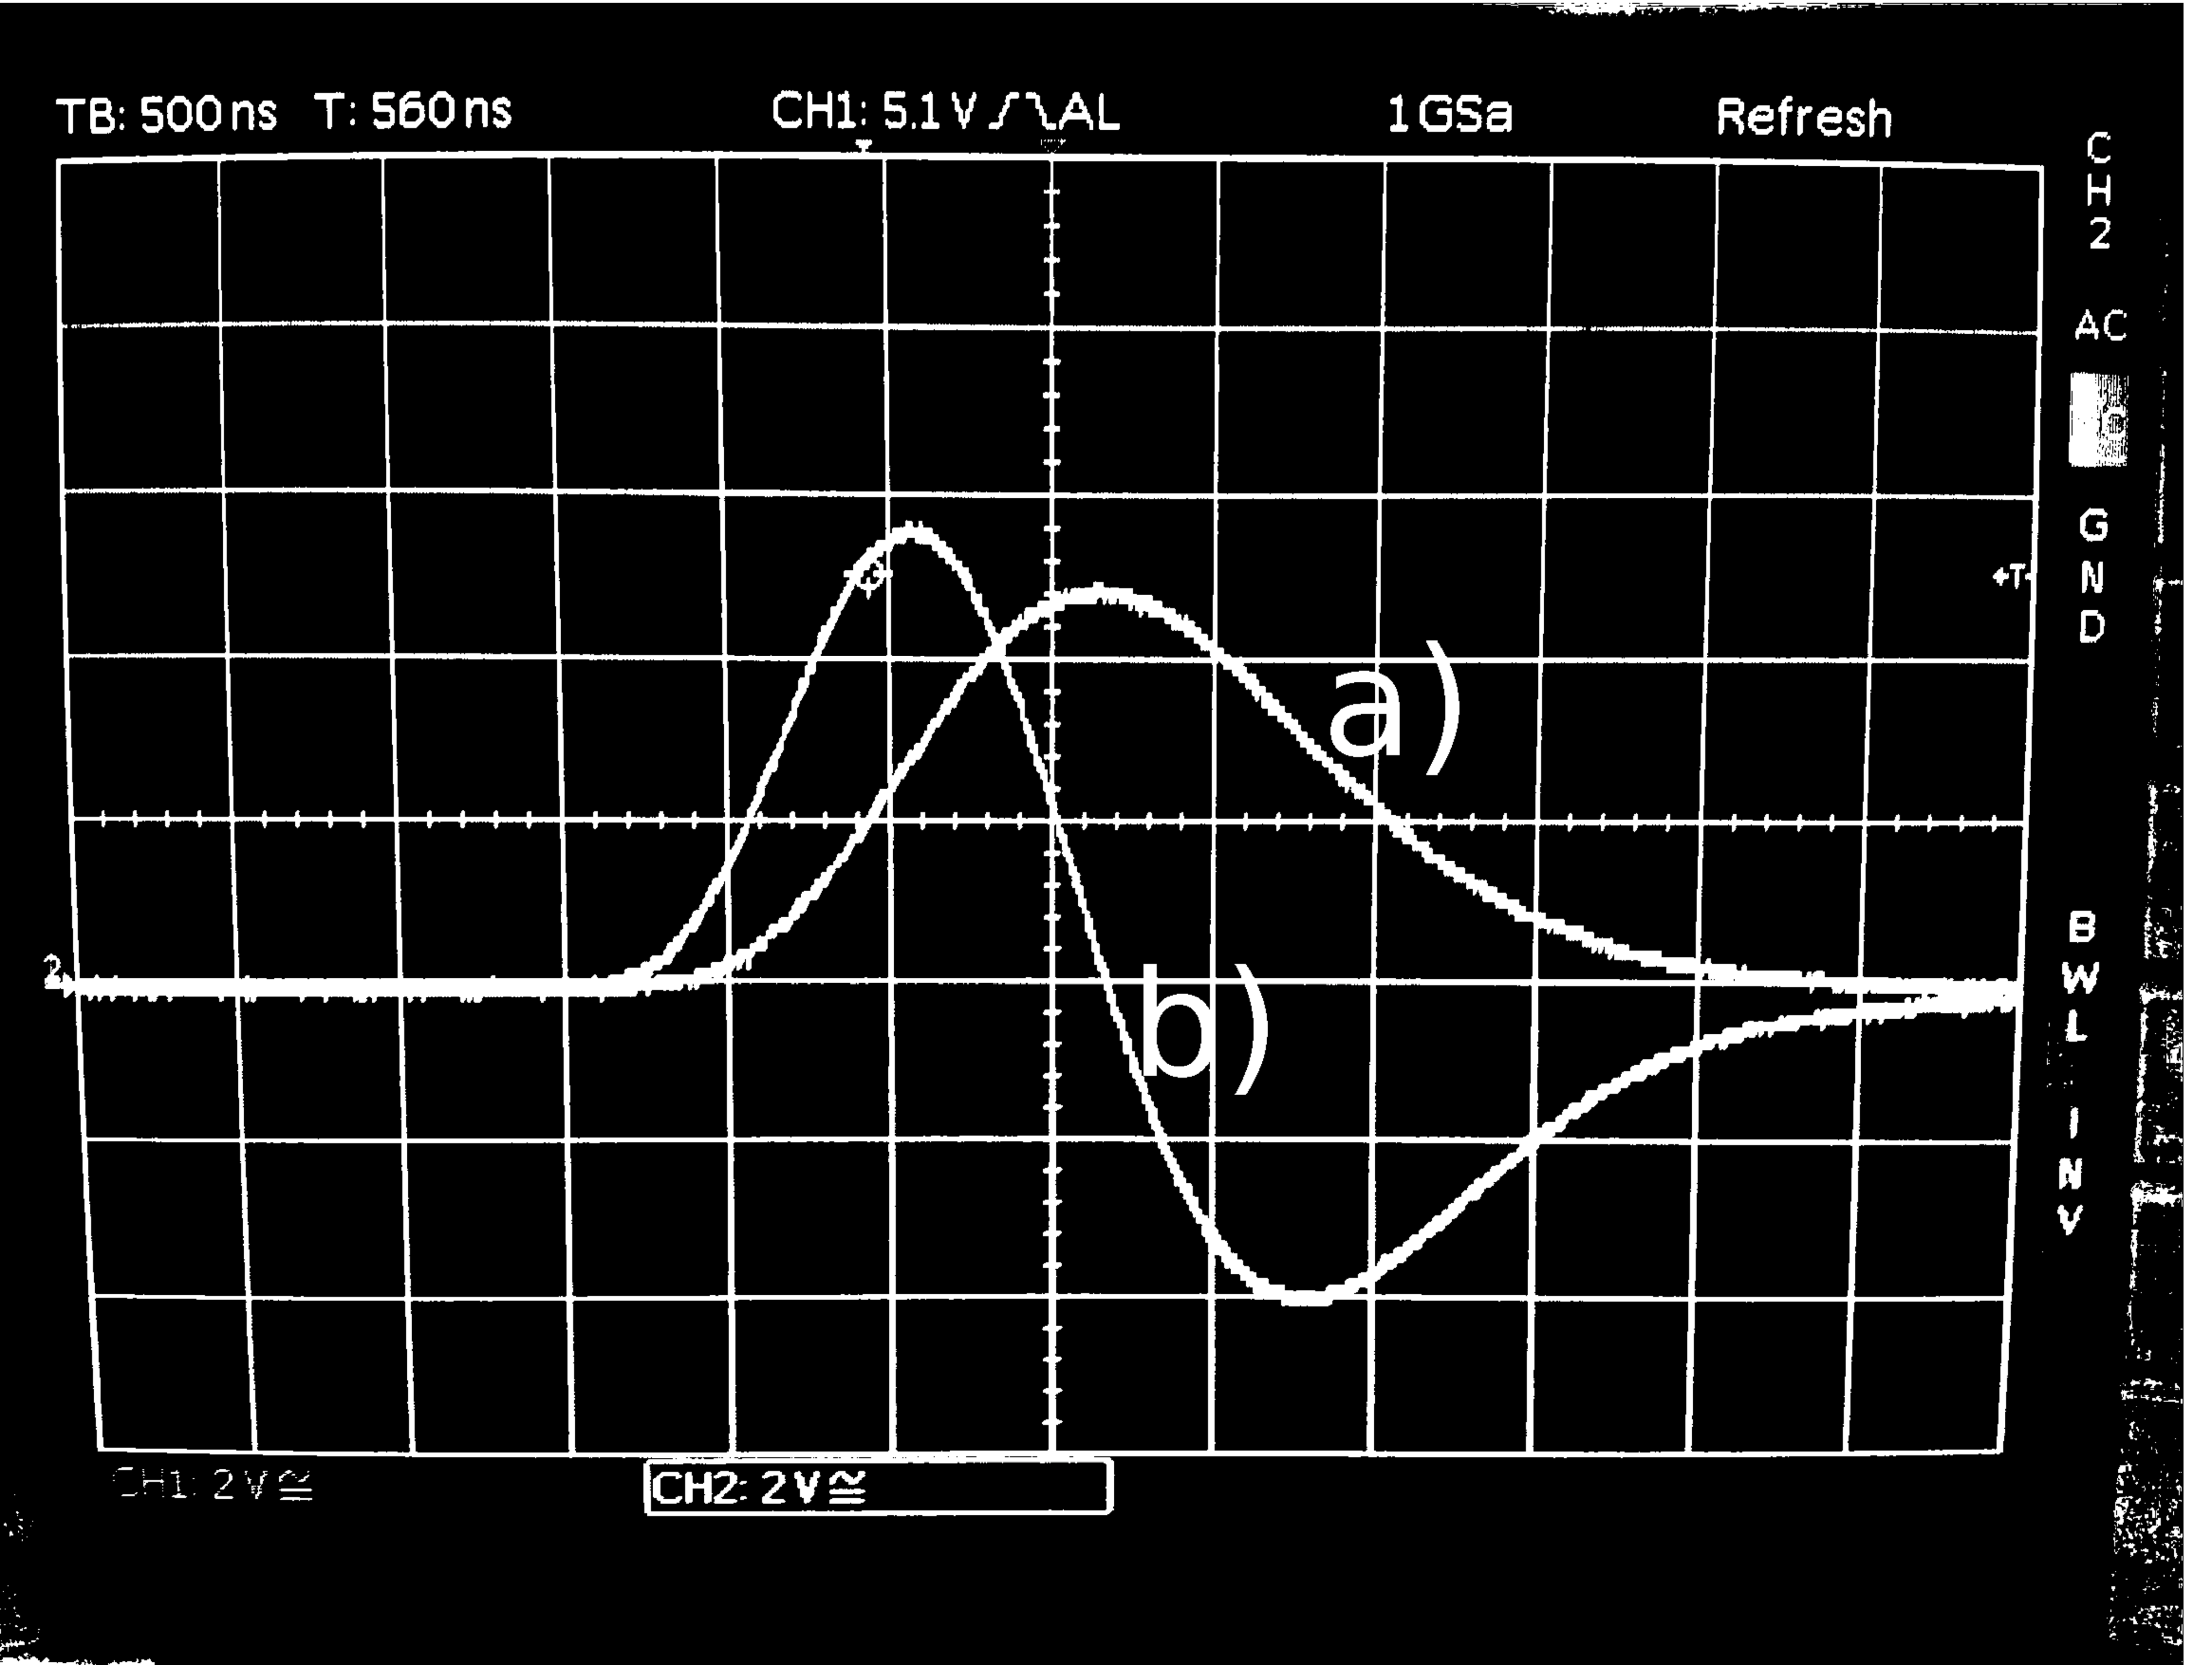
\includegraphics[width=0.8\linewidth]{figures/uni_bipolar2}
    \caption{Signal of the MA on the oscillscope (modified photo), 
        (a) unipolar channel and (b) bipolar channel.}
    \label{fig:uni_bipolar}
\end{figure}

\subsection{Measuring the full energy spectrum}
\label{ssub:Measuring the full energy spectrum}
\paragraph{In the next step,}
we removed the oscilloscope and connected the multichannel analyzer (MA)
in order to measure the energy spectrum. In order to be able to decide which detector and position would
be suitable, we increased gain and coarse gain of the MA to 8.6 and 200, respectively.
This way, the observed spectrum was distributed over the entire range of bins. 
The setup is listed in the appendix, table~\ref{tab:config2}. With the four possible combinations
of position and detector, we obtained four different histograms, shown in figure~\ref{fig:measure2.1}.
For the further measurements, we chose the photomultiplier on the left side for the lower and much less 
pronounced peak, since it show a higher sensibility in that region. The 
chosen position for the sample is thus Pos1, which corresponds to figure~\ref{fig:measure2.1} (a) and (b).

\subsection{Setting the energy window}
\label{ssub:Setting the energy window}
\paragraph{Setting the windows} for the chosen combination of smaple position and detectors did 
not work out right away. In a first attempt, we selected the wrong lower peak (see appendix 
    \ref{sec:appendix_records} for the corresponding settings). 
The second run turned out to be more successful, however. The corresponding configuration is 
shown in the tables below. For the the time delay we chose
$\Delta t = 140$ns.
\begin{figure}[h]
    \centering
    \begin{subfigure}[b]{0.4\linewidth}
        \begin{tabular}{|l|l|}
            \hline
            input           & left detector \\ 
            coarse gain     & 200 \\
            gain            & 8.6 \\
            Shaping time    & $0.5\mu$s \\
            \hline
        \end{tabular}
        \caption{Configuration of MA1}
    \end{subfigure}\qquad
    \begin{subfigure}[b]{0.4\linewidth}
        \begin{tabular}{|l|l|}
            \hline
            input           & MA1, bipolar \\ 
            Lower Level     & $4.75\pm0.05$ \\
            Upper Level     & $3.72\pm0.05$ \\
            Delay           & 1.0 (minimum possible) \\
            \hline
        \end{tabular}
        \caption{Configuration of SCA1}
    \end{subfigure}
    \begin{subfigure}[b]{0.4\linewidth}
        \begin{tabular}{|l|l|}
            \hline
            input           & right detector \\ 
            coarse gain     & 500 \\
            gain            & 8.6 \\
            Shaping time    & $0.5\mu$s \\
            \hline
        \end{tabular}
        \caption{Configuration of MA2}
    \end{subfigure} \qquad
    \begin{subfigure}[b]{0.4\linewidth}
        \begin{tabular}{|l|l|}
            \hline
            input           & MA2, bipolar \\ 
            Lower Level     & $2.02\pm0.05$ \\
            Upper Level     & $3.04\pm0.05$ \\
            Delay           & 1.0 (minimum possible) \\
            \hline
        \end{tabular}
        \caption{Configuration of SCA2}
    \end{subfigure}
    \caption{
        Settings for energy windows. The right detector and thus MA2 and SCA2 is set for the 14.4 keV signal, 
        the left (MA1, SCA1) for the 122 keV signal. Upper and lower level of the SCAs are defined by 
        a potentiometer. The delay of the SCAs was not used. 
        }
    \label{fig:stereo}
\end{figure}

\clearpage
\subsection{Delayed coincidences}
\paragraph{The measurement ran} about 14 hours over night. See Figure~\ref{fig:4_1} for the visualization.
\label{ssub:Conduction of the experiment over night}

\begin{figure}[htpb]
    \centering
    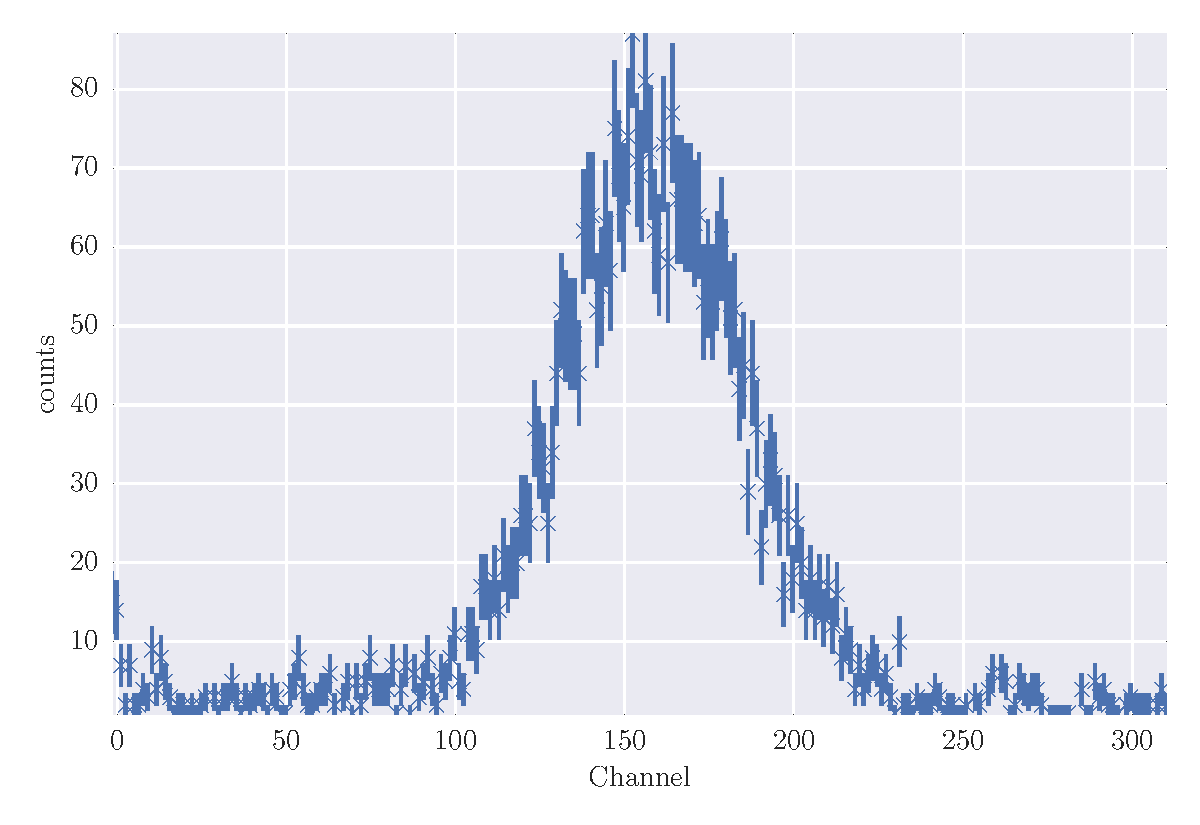
\includegraphics[width=1.0\linewidth]{analysis/figures/plot4_1}
    \caption{Measurement 4.1: One notices that the shape
        of the peak looks gaussian, which is rather unexpected. However,
        further analysis show that the peak is not symmetric and hence the left 
        side will be fitted against a exponential curve, while the origin of the
        right side is the background, which will be analyzed in the next section.
        The errors which are visualized here are approximated by $S_{N_i} = \sqrt{N_i}$, since
        the counts per bin resample a poissonian process.}
    \label{fig:4_1}
\end{figure}
\clearpage
\subsection{Random coicidences}
\label{ssub:Random coicidences}
\paragraph{For measuring the}
background we used the same configuration as before, except of the TAC-input:
\begin{itemize}
    \item TAC Start: SCA2, triggered by the 14.4 keV Peak, delayed with $\Delta t = 48$ns
    \item TAC Stop: SCA1, triggered by 122 keV (no delay)
\end{itemize}
A first approach with $\Delta t = 16$ns failed, since we observed a clear peak in low channels in contrary
to an expected equally distributed signal. After changing to $\Delta t=48$ns the signal looked much more 
like the expected background noise signal (see figure~\ref{fig:5_1}).
\begin{figure}[htpb]
    \centering
    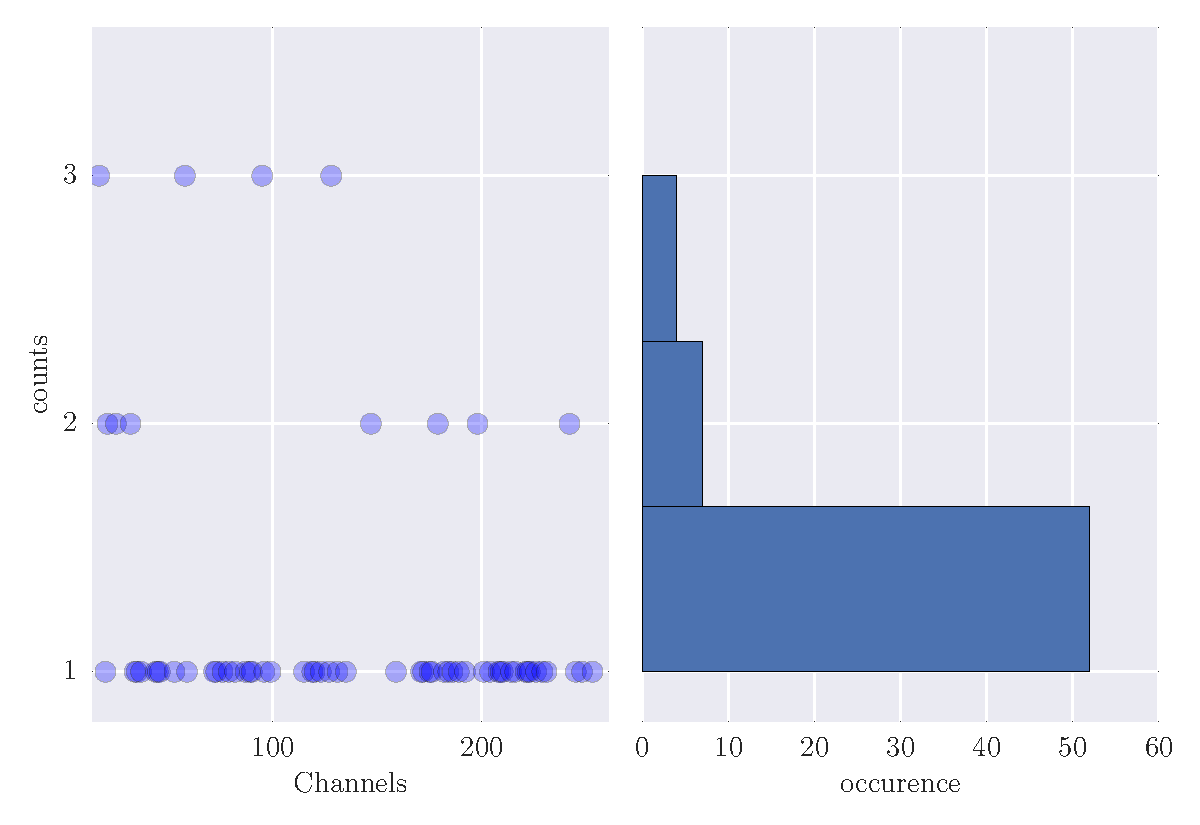
\includegraphics[width=1.0\linewidth]{analysis/figures/plot5_1_hist}
    \caption{
        Measurement 5.1: Result of the background measurement. 
        The left plot shows the recorded histogram (counts per bin). 
        On the right one can observe the distribution of number of counts 
        in one box: It is quite clear that the number of events is much to small 
        to get a decent approximation of the background. Instead of the expected 
        normal distribution around a somewhat higher number of counts, most boxes 
        contain not a single event. 
        }
    \label{fig:5_1}
\end{figure}

\clearpage

